\section{Depth vision}\label{sec:depth-vision}
Depth sensors are devices used to measure the distance between objects and the sensor itself.
This technology has applications in many fields, including robotics, augmented reality (AR), virtual reality (VR),
and computer vision in general.
Depth sensors can be classified according to their principle of operation,
with the main types including infrared sensors, Time-of-Flight (ToF) sensors, and stereo vision sensors.

\subsection{Infrared sensors}\label{subsec:infrared-sensors}
Infrared sensors project a pattern of structured infrared light onto
the scene and capture the reflected image on the infrared receiver.
By analysing the distortion of the pattern caused by objects in the scene,
the sensor is able to compute their distance.
A classic example of this type of sensor is the Microsoft Kinect.

Infrared technology is particularly effective in indoor environments with controlled lighting conditions,
but may be less accurate outdoors or in the presence of strong light sources,
and is also subject to measurement errors that may depend on the material of the objects exposed
to the sensor such as smooth and shiny surfaces~\cite{kinect-resolution}.

\subsection{Time-of-Flight sensors}\label{subsec:time-of-flight-sensors}
Time-of-flight sensors measure the time it takes for emitted light to reach an object and return.
This principle is similar to radar, but uses light instead of radio waves.
An example of a ToF sensor is Microsoft's Kinect v2.

ToF sensors are known for their high accuracy and ability to operate
effectively in outdoor environments, unlike infrared sensors.
However, even these can be affected by the reflectivity of objects and environmental conditions such as fog or rain.

\subsection{Stereo vision sensors}\label{subsec:stereo-vision-sensors}
Stereo vision sensors consist of two or more cameras that are used simultaneously to capture
images of the same scene from slightly different angles, similarly to how human vision works.
The depth in the scene is computed by analysing the differences between the images captured by the different cameras.

Stereo vision sensors are very versatile and can operate in a wide range of environmental conditions,
but require more hardware and more processing power to analyse the captured images.

\subsection{Leap Motion Controller}\label{subsec:leap-motion-controller}
The Leap Motion Controller is a device for hand recognition that uses infrared sensors to accurately
track the position and movement of hands in three dimensions.
The Leap Motion sensor emits infrared light that is reflected by the user's hands and captured by two infrared cameras.
The Leap Motion software processes these images to create a three-dimensional map of the hands and fingers,
enabling natural and intuitive interaction with VR and AR applications.

The Leap Motion is particularly appreciated for its precision and responsiveness,
making it ideal for applications requiring fine control of hand movements.
In the field of augmented reality and virtual reality, Leap Motion is widely used due to its high compatibility with
leading VR and AR viewers such as the Oculus Rift, HTC Vive, Pico and Varjo.

This versatility makes it a popular option for developing applications in a variety of fields
beyond the gaming and entertainment industry,
including the medical field, in particular physical and cognitive rehabilitation~\cite{leap-motion-rehab-1, leap-motion-rehab-2},
social skills development for people with autism~\cite{leap-motion-autism-1, leap-motion-autism-2},
education and training in various disciplines~\cite{leap-motion-anatomy-education, leap-motion-boolean-logic-education,
	leap-motion-music-education, leap-motion-medical-education},
and sign language recognition~\cite{leap-motion-sign-language-1, leap-motion-sign-language-2}.

The Leap Motion Controller is the device used in the very first prototype of this project~\cite{keyrtual}.

\begin{figure}[ht]
	\begin{subfigure}{.3\textwidth}
		\center
		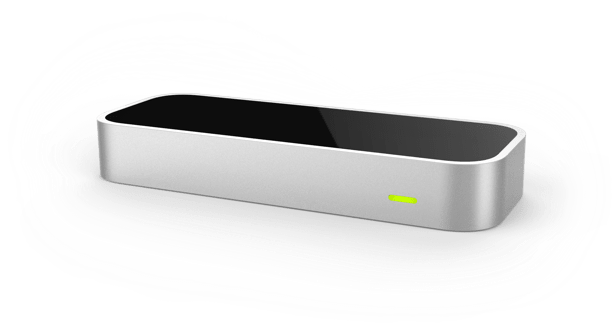
\includegraphics[width=\textwidth]{leap-motion}
	\end{subfigure}
	\begin{subfigure}{.3\textwidth}
		\center
		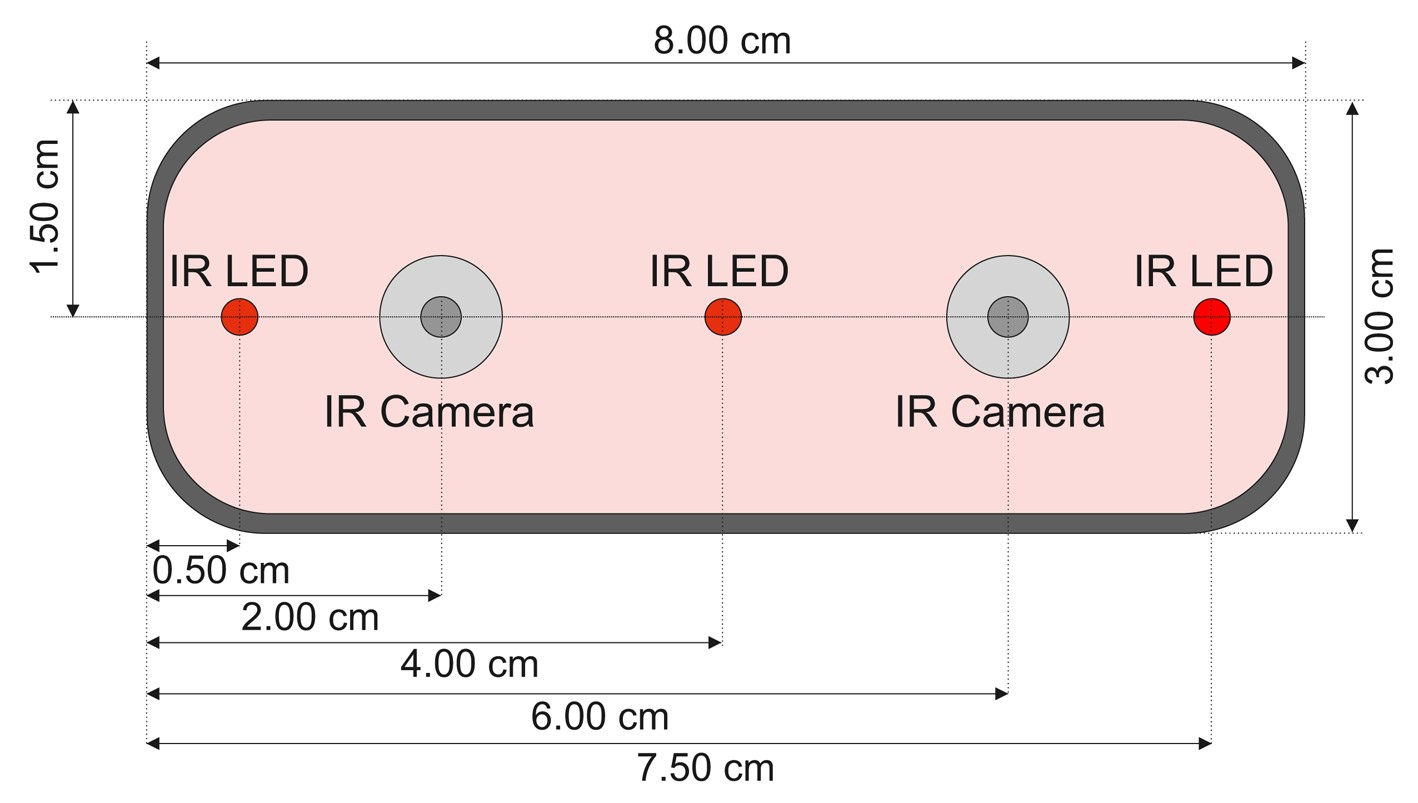
\includegraphics[width=\textwidth]{leap-motion-components}
	\end{subfigure}
	\begin{subfigure}{.3\textwidth}
		\center
		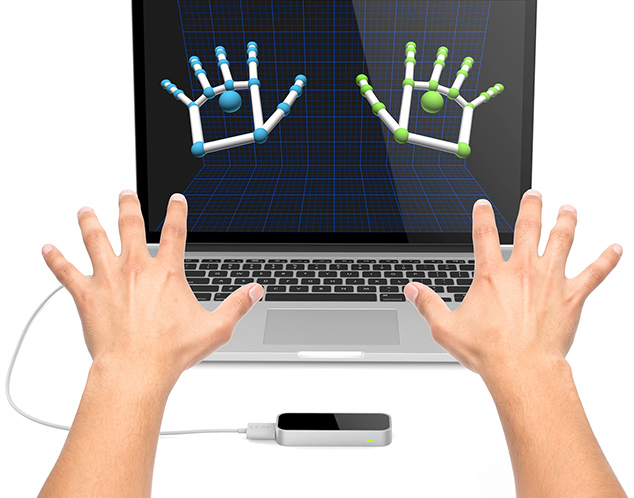
\includegraphics[width=\textwidth]{leap-motion-usage}
	\end{subfigure}
	\caption{Leap Motion Controller, sensors \protect\cite{leap-motion-components-image} and usage}
	\label{fig:leap-motion-components}
\end{figure}

\subsection{Kinect}\label{subsec:kinect}
The Microsoft Kinect is probably one of the best known and most widely used depth sensors.
It exists in two versions, which use different technologies to measure depth.
The first version of the Kinect used structured infrared light technology to create a depth map with a
resolution of $640 \times 480$ pixels and a frequency of 30 FPS~\cite{kinect-v1-and-v2-technical-info},
while the second version, the Kinect v2, uses a ToF sensor with a resolution of $512 \times 424$
pixels~\cite{kinect-v1-and-v2-technical-info} and a frequency of 30 FPS~\cite{kinect-v2-fps}.

The Kinect was originally designed for the Xbox 360 gaming console, but quickly became a popular
tool in research and development of interactive applications due to its ability to track human
body movements in real time and the dual presence of an infrared depth sensor and an RGB camera.

The Kinect has found applications in many areas beyond the video game industry, including
education~\cite{kinect-power-point, kinect-engineering, kinect-manipulation-3D-objects},
robotics~\cite{kinect-robot-1, kinect-robot-2},
and surveillance~\cite{kinect-surveillance-1, kinect-surveillance-2}.

\begin{figure}[ht]
	\begin{subfigure}{.5\textwidth}
		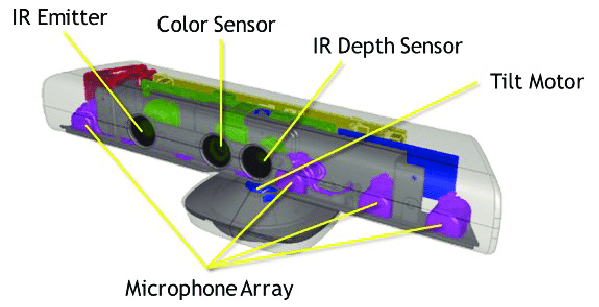
\includegraphics[width=\textwidth]{kinect-components}
	\end{subfigure}
	\begin{subfigure}{.5\textwidth}
		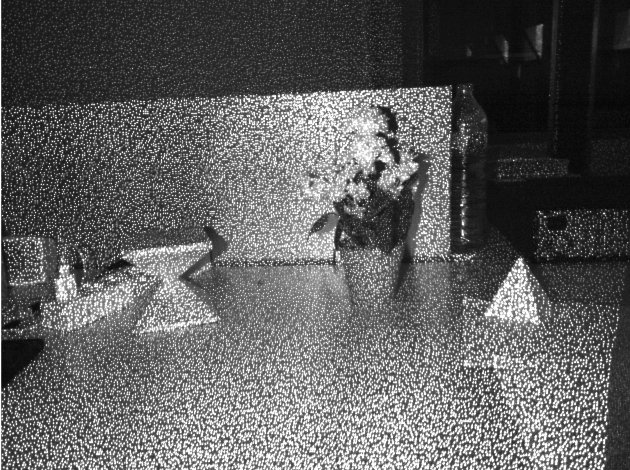
\includegraphics[width=\textwidth]{structured-light-kinect}
	\end{subfigure}
	\caption{Microsoft Kinect components \protect\cite{kinect-components-image} and structured light pattern \protect\cite{structured-light-kinect}}
	\label{fig:kinect-components}
\end{figure}

\subsection{RealSense}\label{subsec:realsense}
Intel's RealSense sensor line uses a combination of technologies,
including stereo vision and ToF, to provide high-resolution depth data.
RealSense sensors are designed to be integrated into a wide range of devices,
from drones to robots to AR and VR devices, thanks in part to the robust SDK developed by Intel,
which facilitates integration and custom application development.

RealSense sensors capture both depth images,
with a resolution of up to $1280 \times 720$ pixels and a frame rate of 90 FPS~\cite{realsense-resolution},
and RGB images, with a resolution of up to $1920 \times 1080$ pixels and a frame rate of 30 FPS~\cite{realsense-resolution}.

The ability of RealSense sensors to capture detailed depth maps makes them
ideal for 3D mapping applications even in outdoor environments~\cite{realsense-mapping}.
Among other fields of application, RealSense sensors are widely used in face detection
and its applications such as facial expression recognition~\cite{realsense-expressions},
3D face reconstruction~\cite{realsense-face-reconstruction},
and face detection~\cite{realsense-face-detection}.

\begin{figure}[ht]
	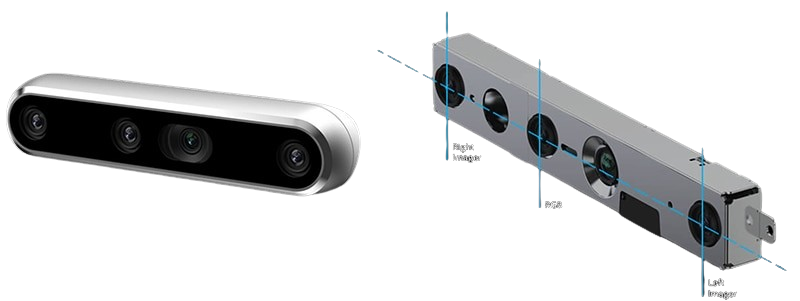
\includegraphics[width=\textwidth]{realsense}
	\caption{RealSense components}
	\label{fig:realsense-components}
\end{figure}


